\documentclass{article}
\usepackage{amssymb}
\usepackage{courier}
\usepackage{fancyhdr}
\usepackage{fancyvrb}
\usepackage[T1]{fontenc}
\usepackage[top=.75in, bottom=.75in, left=.75in,right=.75in]{geometry}
\usepackage{graphicx}
\usepackage{lastpage}
\usepackage{listings}
\lstset{basicstyle=\small\ttfamily}
\usepackage{soul}
\usepackage{upquote}
\usepackage{xcolor}

\usepackage[colorlinks,urlcolor={blue}]{hyperref}

\begin{document}

\fancyfoot[L]{\color{gray} C4CS -- W'16}
\fancyfoot[R]{\color{gray} Revision 1.0}
\fancyfoot[C]{\color{gray} \thepage~/~\pageref*{LastPage}}
\pagestyle{fancyplain}


\title{\textbf{Advanced Homework 5\\}}
\author{Assigned: Friday, February 5, 11:00AM}
\date{\textbf{\color{red}{Due: Before the first lecture on Friday, February 19}}}
\maketitle


\section*{Submission Instructions}
To receive credit for this assignment you will need to stop by someone's
office hours, demo your running code, and answer some questions.

\section{Automated Background Testing with Git Hooks}

As projects grow, the number and complexity of test cases grows as well. While
it's generally a good idea to run all of your test cases, it can be annoying
to sit around and wait for a long test case that tests a part of your program
that (you think) you didn't touch.

\medskip
\noindent
Hooks and scripting to the rescue! The goal is to write a post-commit hook
that runs in the background. This script will make sure everything builds
correctly, run all of your tests, and, as a bonus, run an external correctness
checker that can help find mistakes.

\medskip
\noindent
First read over everything your script should do:

\begin{enumerate}
  \item Create a directory in /tmp that is unique for this project if one does not already exist
    \begin{itemize}
      \item \small \em Hint: The project's current directory is already unique
    \end{itemize}
  \item Assuming the directory you created above is at \texttt{\$PROJ\_TMP\_DIR}, run
    \begin{itemize}
      \item \texttt{git clone -{}-local .\ \$PROJ\_TMP\_DIR/\$(git describe -{}-always)}
    \end{itemize}
  \item Call a second script that runs in the background to execute the
    remaining tasks. This second script should do all of its work in the clone
    you just made.
    \begin{itemize}
      \item \small \em Hint: You will likely need to pass arguments to this secondary script
    \end{itemize}
  \item Call \texttt{make} to build the project. You should save all of the
    regular output to a file named \texttt{build.log} and any errors to a file
    named \texttt{build.error}
    \begin{itemize}
      \item If the build fails, your script should stop and notify that the
        build failed. See the notify section below.
    \end{itemize}
  \item Run every test case for this project
    \begin{itemize}
      \item Your script should assume that any executable file with ``test''
        in the name is a test case. It should \textbf{not} hard-code a list of
        tests to run
      \item Your script should save the regular output and the error output of
        each test case to unique files.
      \item Your script should assume that test cases return 0 when they
        pass and non-zero otherwise.
    \end{itemize}
  \item Run the \texttt{cppcheck} utility for this project
    \begin{itemize}
      \item \emph{\small You will need to install this utility first
        (\texttt{sudo~apt-get~install~cppcheck}), your script may assume that
        cppcheck is already installed}
      \item \texttt{cppcheck} is a style and correctness checker (it is a
        \emph{linter} and a \emph{static analysis} tool).
      \item You should invoke \texttt{cppcheck} as
        ``\texttt{cppcheck~--enable=all~.}'' (try it out!)
      \item You should again save the regular output and error output into
        separate files.
    \end{itemize}
  \item Generate a nice report when everything is done and alert the user
    using \texttt{notify-send}\\
    \begin{minipage}{0.6\textwidth}
      \begin{itemize}
        \item Try running \texttt{notify-send "I am a title" "And I am a body"}
        \item This is an example of my notification. You don't need to match my
          formatting, simply include in the notification what you think is
          useful. At a minimum it should include (a) how many test cases passed,
          and (b) if the style checker reported any warnings.
      \end{itemize}
    \end{minipage}
    \hfill
    \begin{minipage}{0.3\textwidth}
      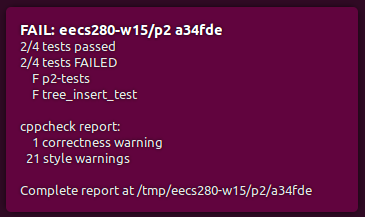
\includegraphics[width=\linewidth]{notification}
    \end{minipage}
\end{enumerate}

\medskip
\noindent
Notice that this hook is \textbf{generic}. It should work in any repository
simply by copying both scripts into the \texttt{.git/hooks} directory.

\bigskip
\hrule
\bigskip

\medskip
\noindent
To get started, use the EECS\,280~W15 repository you created for Homework~4.

\medskip
\noindent
Create a directory to hold the hooks you're working on
\begin{itemize}\tt
  \item mkdir \textasciitilde/hooks
\end{itemize}
This is going to be a kinda complicated script, so it's a good
idea to put it under version control as well.
\begin{itemize}\tt
  \item cd \textasciitilde/hooks
  \item git init
\end{itemize}
Inside this directory, create a file named \texttt{post-commit} with the
following contents.  Also be sure to make this script executable.
\begin{lstlisting}
#!/usr/bin/env bash

echo "Hello, I am your commit hook running."

echo "Number of arguments I received: $#"
echo "Argument[0] (the program being run): $0"
echo "Argument[1]: $1" # This is empty if no arguments were passed
echo "Argument[2]: $2" # This is empty if only one argument was passed

# Notice what directory this script is executed from. This is important
# when you try to call your helper script
echo "$(pwd)"

sleep 10s && echo "It is annoying to wait for long commit hooks to finish"

sleep 10s & echo "We can put them in background them however so we don't have to wait"

notify-send "Test Message" "Blocking part of the commit hook finished"

echo "Notice that the second sleep is still running, we can tell by: $(pidof sleep)"
\end{lstlisting}
%
Don't forget to add and commit the starter code
\begin{itemize}\tt
  \item git add post-commit
  \item git commit
\end{itemize}
%
Now, go to the git repository you created in Homework~4 and install this hook
\begin{itemize}\tt
  \item cd \textasciitilde/eecs280-w15/p2/.git/hooks~~~\#\,Or wherever you put this
  \item ln -s \textasciitilde/hooks/post-commit .
\end{itemize}
The command \texttt{ln -s} creates a symbolic link, or symlink. Recall
symlinks are just like pointers. This design lets us install the same commit
hook into multiple repositories just by pointing to it. If we ever update or
make improvements to the hook, all of the repositories that use it will
automatically get upgraded.

\medskip
\noindent
All right, we are finally set up. Make a new commit and test out the new hook!

\newpage

\subsection*{Some final tips}

\begin{itemize}
  \item Build up your solution in parts. Get step 1 working then commit it.
    Then onto step 2.
  \item Steps 1 and 5 are probably the most challenging. Step 6 is almost an
    exact copy of step 4.
  \item You, of course, do not need to actually implement project~2 from
    EECS\,280.  I recommend something like this:%
\lstset{basicstyle=\footnotesize\ttfamily}
\begin{lstlisting}
ppannuto@ppannuto-c4cs-vm:~/hw4> git log --oneline -n1 -p
dfaeb04 Force filter_test to always succeed
diff --git a/filter_test.cpp b/filter_test.cpp
index eebeb87..fa1bc1e 100644
--- a/filter_test.cpp
+++ b/filter_test.cpp
@@ -20,6 +20,7 @@ bool isPrime(int x)
 
 int main()
 {
+    return 0;
     int numbers[] = { 3, 20, 46, 43, 9, 17, 103, 102 };
     const int numSize = sizeof(numbers) / sizeof(int);
     int primes[] = { 3, 43, 17, 103 };
\end{lstlisting}
\end{itemize}


\subsection*{Submission checkoff:}
\begin{itemize}
  \item[$\square$] Explain what the clone command from step~2 does.
  \item[$\square$] Show off your hook working
    \begin{itemize}
      \item[$\square$] With all passing test cases
      \item[$\square$] With some failing test cases
      \item[$\square$] Show how to find and examine the output from a failing
        test case
    \end{itemize}
  \item[$\square$] Show that your hook is generic by installing it (symlinking
    it) into a repository for an EECS class you are currently taking
    \begin{itemize}
      \item If you aren't in a programming EECS class, grab
        \href{http://www.andrewdeorio.com/teaching/eecs280/}{any other 280
        project from W15}.
    \end{itemize}
\end{itemize}

\end{document}
